\subsection{Paraphrasing Chunks}
\label{subsec:paraphrasing_chunks}

We wanted to evaluate whether chunk-to-chunk paraphrases exhibit better control than text-to-text paraphrases, since chunks are shorter than text and contain fewer topic changes in theory.
We use five texts from the \dataBlog{}, \dataGutenberg{}, and the \dataStudent{} dataset.
There are two steps to this experiment: (1) generating chunks and their respective paraphrases, (2) 

When chunking texts, we preserved sentences via using \texttt{nltk}'s \texttt{sent\_tokenize}.
We grouped sentences in order and such that each chunk roughly contains the same number of words.
We tested the detector performance for 1 to 5 chunks per text across all \imp{} generation models, on two prompts for one-tep paraphrasers and on two temperatures for two-step paraphrasers.
Each paraphraser returns one paraphrase per configuration.

\begin{figure}[ht]
  \centering
\resizebox{\textwidth}{!}{%
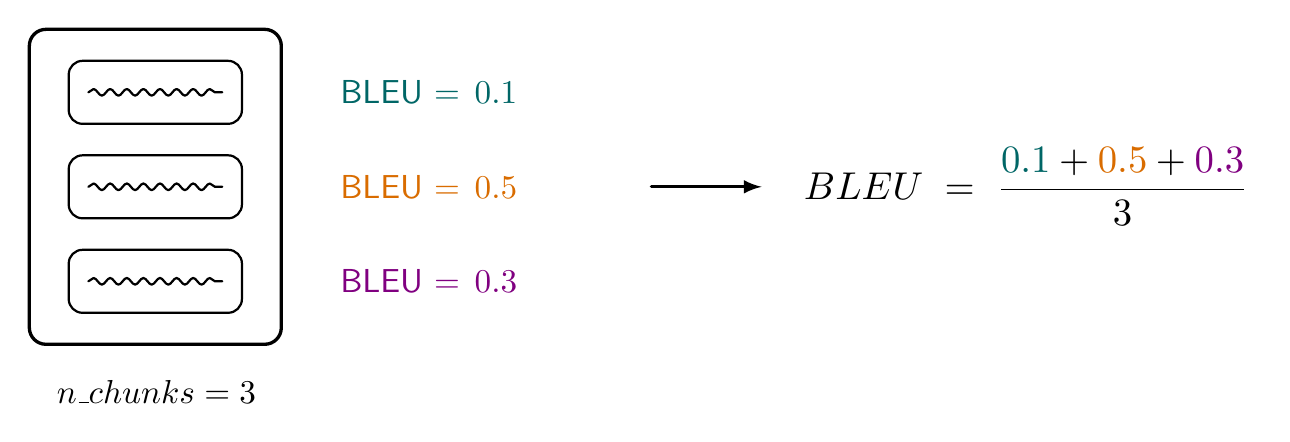
\begin{tikzpicture}[line join=round,line cap=round, >=latex, font=\sffamily]

% --- Left black container with three chunks ---
\draw[black, very thick, rounded corners=6pt]
  (-0.2,3.6) rectangle (3.0,-0.4);

% three inner rounded rectangles
\foreach \y in {2.8,1.6,0.4}{
  \draw[black, thick, rounded corners=5pt] (0.3,\y+0.4) rectangle (2.5,\y-0.4);
  % squiggle inside
  \draw[black, thick, decorate, decoration={snake,amplitude=1.2pt,segment length=6pt}]
    (0.55,\y) -- (2.25,\y);
}

% --- Colored BLEU labels next to each chunk ---
\node[anchor=west, text=teal!80!black, scale=1.2]  at (3.6,2.8) {BLEU $=\,0.1$};
\node[anchor=west, text=orange!85!black, scale=1.2] at (3.6,1.6) {BLEU $=\,0.5$};
\node[anchor=west, text=violet, scale=1.2]         at (3.6,0.4) {BLEU $=\,0.3$};

% --- n_chunks = 3 (black) ---
\node[anchor=west, text=black, scale=1.2] at (0.0,-1.0) {$n\_\text{chunks}=3$};

% --- Arrow to the right and mean BLEU expression ---
\draw[black, very thick, ->, >=latex] (7.7,1.6) -- (9.1,1.6);

\node[anchor=west, text=black, scale=1.4] at (9.3,1.6)
  {$\varnothing\ \text{BLEU} \;=\; \displaystyle
   \frac{\textcolor{teal!80!black}{0.1}+\textcolor{orange!85!black}{0.5}+\textcolor{violet}{0.3}}{3}$};

\end{tikzpicture}
}
  \caption{Computation of the mean \ac{bleu} score over 3 text chunks.}
  \label{fig:mean-bleu}
\end{figure}

For each configuration, we compute BERTScore Precision, BERTScore Recall, BERTScore F1, SBERT \ac{wms}, SBERT cosine similarity, ROUGE1, ROUGE2, ROUGEL, ROUGELsum, BLEU, and METEOR.
